\documentclass{beamer}
\usepackage[english]{babel}
\usepackage[utf8]{inputenc}
\usepackage{graphicx}
\usepackage{amsfonts}

\author{Maarten de Jonge}
\title[PGA]{Projective 2D Line Geometry using Geometric Algebra}
\subtitle{Supervisor: Leo Dorst}

\newcommand{\rp}{$\mathbb{R}^{3,3}$}

\begin{document}

  \frame{\titlepage}
  
  \begin{frame}
    \frametitle{Projective Geometry}
    The branch of geometry concerned with properties that are
    invariant under projective transformations. That means:

    \begin{itemize}
      \item No
        \begin{itemize}
          \item distances
          \item angles
        \end{itemize}
      \item Yes 
        
        \begin{itemize}
          \item intersections
          \item tangents
        \end{itemize}
    \end{itemize}
    
    Has various applications in areas such as computer vision.
  \end{frame}

  \begin{frame}
    \frametitle{Line Geometry in Terms of the Null
Geometric Algebra over \rp\cite{hangbo2011}}
    Conic sections are represented as a cross-section of a \emph{regulus}.
    \begin{center}
      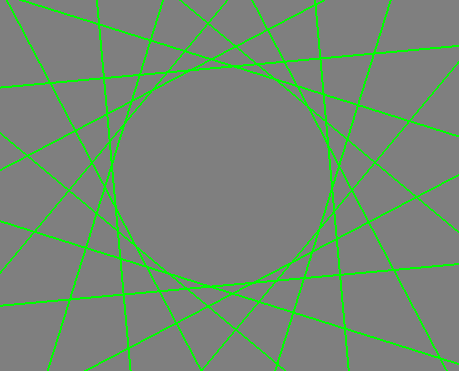
\includegraphics[width=0.7\textwidth]{circle.png}
    \end{center}
  \end{frame}

  \begin{frame}
    \frametitle{Line Geometry in Terms of the Null
Geometric Algebra over \rp\cite{hangbo2011}}
    Conic sections are represented as a cross-section of a \emph{regulus}.
    \begin{center}
      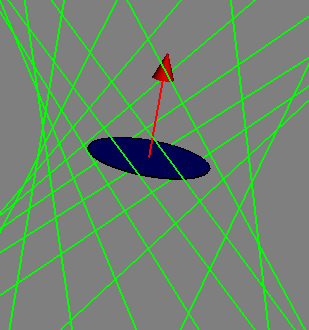
\includegraphics[width=0.7\textwidth]{axis.png}
    \end{center}
  \end{frame}
  

  \begin{frame}
    \frametitle{Problems}
    \begin{itemize}
      \item There is no way to visualise/interpret a general regulus yet.
      \item How to represent the 2D geometry in a line-based fashion?
        e.g.
        \begin{itemize}
          \item obtain a point on a conic section
          \item obtain a conic section given a number of points
            and/or tangent lines
        \end{itemize}
    \end{itemize}
  \end{frame}
  
  \begin{frame}
    \frametitle{Progress}
    
    \begin{itemize}
      \item Regulus visualisation is really almost done this time.
        \begin{itemize}
          \item most of the things which can be overlooked have been
            overlooked by now
        \end{itemize}
    \end{itemize}
    Problems faced:
    \begin{enumerate}
      \item Large complex codebase which takes getting used to
      \item Drawing is done using OpenGL; uncomfortable conversions
        from GA to LA
      \item Lack of mathematical experience leads to silly mistakes.
    \end{enumerate}
  \end{frame}

  \begin{frame}
    \frametitle{Progress}
    
    \begin{itemize}
    \item Have started preparing for the geometry that follows.
    \end{itemize}
    \begin{center}
      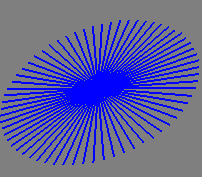
\includegraphics{point.png}
    \end{center}
  \end{frame}

\bibliographystyle{apalike}
\begin{frame}
  \frametitle{References}
  \bibliography{library}
\end{frame}
\end{document}
